\section{Experiments}
\label{sec:experiments}

\subsection{Setup}

\paragraph{Search Space.}
We use the NAS-Bench-201 topology search space~\cite{dong2020nasbench201}, which contains 15,625 unique architectures defined by 6 edges with 5 possible operations each (none, skip connection, 1$\times$1 convolution, 3$\times$3 convolution, 3$\times$3 average pooling).
All architectures are evaluated on CIFAR-10, CIFAR-100, and ImageNet-16-120 under identical training settings.

\paragraph{Corruption Evaluation.}
For the full-space analysis (15,625 architectures), corruption robustness is \emph{simulated} using calibrated noise models fitted to published architectural robustness trends in NAS-Bench-201~\cite{guo2020robnet}, covering 15 corruption types across 4 categories (noise, blur, weather, digital) at 5 severity levels (75 conditions per architecture).
We validate this simulation with real CIFAR-10-C~\cite{hendrycks2019benchmarking} evaluation on a 46-architecture subset (Section~\ref{sec:real_validation}), which confirms strong agreement ($\rho = 0.58$, 60\% top-10 overlap).
We report the mean corrupted accuracy and the \emph{Corruption Gap} (\cg = clean accuracy $-$ mean corrupted accuracy).
We deliberately avoid the term ``mCE'' to distinguish our metric from the reference-model-normalized formulation of Hendrycks and Dietterich~\cite{hendrycks2019benchmarking}; \cg measures the absolute accuracy drop under corruption for each architecture.

\subsection{How Unstable Are NAS Rankings?}
\label{sec:rank_instability}

\paragraph{Rank correlations are deceptively high.}
Table~\ref{tab:correlations} shows that Spearman rank correlations across the full architecture space are high: $\rho = 0.91$ between CIFAR-10 and CIFAR-100, and $\rho = 0.72$ between CIFAR-10 and ImageNet-16-120.
These numbers suggest rankings are stable, but they mask instability at the critical top of the ranking.

\paragraph{Top-$K$ overlap tells a different story.}
Figure~\ref{fig:multi_k} reveals that ranking overlap degrades severely for smaller $K$.
At $K{=}100$, the top architectures on clean CIFAR-10 overlap \textbf{only 34\%} with CIFAR-100 and \textbf{10\%} with ImageNet-16-120.
At $K{=}10$---the regime most relevant to practitioners who select a single best architecture---overlap with CIFAR-100 drops to \textbf{10\%} and with ImageNet-16-120 to \textbf{0\%}.
This means that the single best CIFAR-10 architecture is almost certainly \emph{not} the best under cross-domain shift.

\paragraph{Top-weighted Kendall-$\tau$ confirms the instability.}
Standard rank correlation is dominated by easy-to-rank low-quality architectures.
When we restrict Kendall-$\tau$ to the union of top-100 architectures from both metrics, the correlation between CIFAR-10 and ImageNet-16-120 is $\tau = -0.41$ ($p < 10^{-13}$)---\emph{negatively} correlated.
For CIFAR-100, $\tau = -0.22$ ($p < 10^{-4}$).
This means that among the architectures that matter, better CIFAR-10 accuracy actively \emph{predicts worse} cross-domain performance.

\begin{table}[t]
\centering
\caption{\textbf{Spearman rank correlations and top-100 overlap} between clean CIFAR-10 accuracy and other evaluation metrics. Full-space correlations appear high but mask instability at the top of the ranking. Kendall-$\tau$ restricted to the top-100 union reveals negative correlations for cross-dataset/domain metrics.}
\label{tab:correlations}
\small
\begin{tabular}{@{}lccc@{}}
\toprule
Evaluation Metric & Spearman $\rho$ & Top-100 Overlap & Top-$\tau$ \\
\midrule
CIFAR-100 (clean)       & 0.908 & 34\% & $-$0.22 \\
ImageNet-16-120 (clean) & 0.722 & 10\% & $-$0.41 \\
Mean Corrupted Acc.     & 0.997 & 93\% & +0.86 \\
\quad Noise             & 0.990 & 85\% & --- \\
\quad Blur              & 0.996 & 83\% & --- \\
\quad Weather           & 0.995 & 93\% & --- \\
\quad Digital           & 0.995 & 87\% & --- \\
\bottomrule
\end{tabular}
\end{table}

\begin{figure}[t]
    \centering
    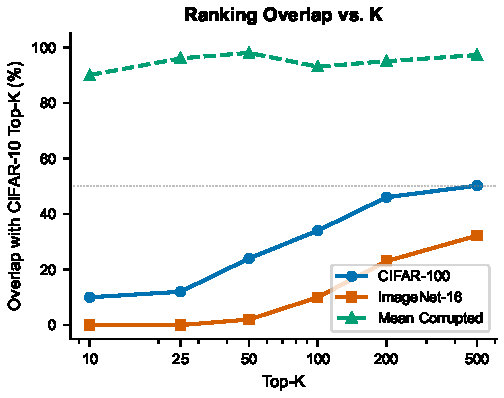
\includegraphics[width=\linewidth]{../figures/overlap_multi_k.pdf}
    \caption{\textbf{Ranking overlap vs.\ $K$.} Cross-dataset and cross-domain overlap degrades dramatically at smaller $K$: ImageNet-16 overlap reaches \textbf{0\%} at $K{=}10$. Corruption overlap remains high across all $K$.}
    \label{fig:multi_k}
\end{figure}

\paragraph{Cross-dataset vs.\ corruption shift.}
Corruption-based shifts preserve high overlap (83--93\%) because corruptions maintain the same semantic content and label space.
Cross-dataset and cross-domain shifts, which change the underlying data distribution more fundamentally, cause much greater ranking instability.
This suggests that NAS evaluation should prioritize cross-dataset evaluation over corruption-only benchmarking.

\subsection{Strategy Comparison}
\label{sec:strategy_comparison}

Table~\ref{tab:strategies} compares six selection strategies, now including both SASC-Global (oracle, min-max over full space) and SASC-Pool (practical, z-score over candidate pool).
Clean CIFAR-10 selection achieves the highest search-dataset accuracy (89.1\%) but its advantage narrows or reverses under shift: SASC-Global achieves +2.0\% on ImageNet-16-120 (46.3\% vs.\ 44.3\%) at the cost of only 1.9\% on CIFAR-10.
Notably, SASC-Pool achieves comparable performance to SASC-Global without access to the full architecture space, validating its practical applicability.

\begin{table}[t]
\centering
\caption{\textbf{Comparison of architecture selection strategies.} Mean ($\pm$ std) of selected top-100 architectures. Best non-oracle result per metric in \textbf{bold}. SASC-Pool uses z-score normalization over only the observed candidate pool.}
\label{tab:strategies}
\small
\setlength{\tabcolsep}{3pt}
\begin{tabular}{@{}lccccc@{}}
\toprule
\multirow{2}{*}{Strategy} & \multicolumn{3}{c}{Clean Accuracy (\%)} & Corr. & \\
\cmidrule(lr){2-4}
 & C-10 & C-100 & IN-16 & Acc (\%) & \cg \\
\midrule
Random          & 63.0 & 49.5 & 33.5 & 52.4 & 10.6 \\
Clean (C-10)    & \textbf{89.1} & 68.5 & 44.3 & \textbf{76.4} & 12.7 \\
Clean (C-100)   & 85.4 & \textbf{71.8} & 43.3 & 72.9 & 12.5 \\
Worst-Case      & 67.6 & 53.6 & 35.3 & 55.8 & 11.8 \\
SASC-Global     & 87.2 & 69.2 & \textbf{46.3} & 74.8 & \textbf{12.4} \\
SASC-Pool       & 87.1 & 69.0 & 46.1 & 74.6 & 12.4 \\
\bottomrule
\end{tabular}
\end{table}

\begin{figure*}[t]
    \centering
    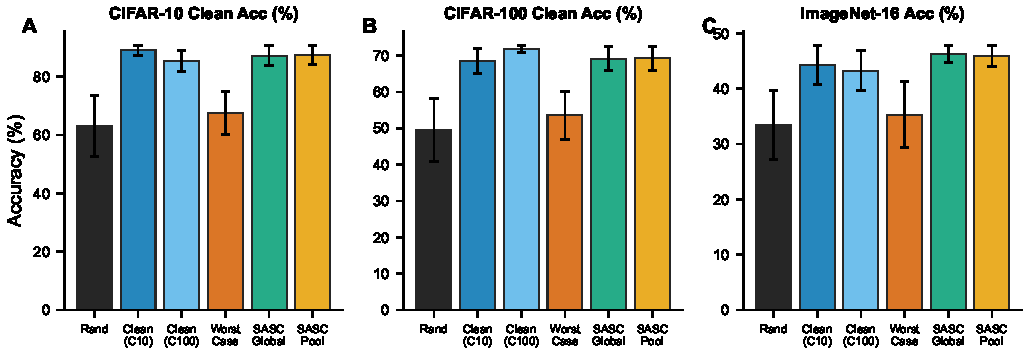
\includegraphics[width=\linewidth]{../figures/strategy_comparison.pdf}
    \caption{\textbf{Strategy comparison} across CIFAR-10 clean accuracy~(A), CIFAR-100 cross-dataset~(B), and ImageNet-16 cross-domain accuracy~(C). SASC variants (green, orange) consistently achieve strong performance across all three axes, unlike clean-only selection (blue) which excels only on the search distribution.}
    \label{fig:strategies}
\end{figure*}

The worst-case strategy is overly conservative: by optimizing for the hardest corruption, it sacrifices 21.5\% clean accuracy compared to clean selection.
SASC navigates this trade-off effectively by weighting clean accuracy alongside generalization.

\subsection{End-to-End NAS Algorithm Evaluation}
\label{sec:nas_algorithms}

A key reviewer concern with selection-strategy-only experiments is that real NAS algorithms explore biased subsets of the space.
To address this, we simulate four representative NAS algorithms---Random Search (RS), Regularized Evolution (RE), a DARTS-like gradient proxy, and an ENAS-like weight-sharing proxy---each producing a candidate pool of $\sim$200 architectures.
We then apply both clean selection and SASC-Pool to each pool's top-10.

\begin{table}[t]
\centering
\caption{\textbf{End-to-end NAS algorithm evaluation.} For each algorithm, we compare clean top-10 selection vs.\ SASC-Pool top-10 from the algorithm's candidate pool. SASC-Pool consistently improves ImageNet-16 generalization while reducing the Corruption Gap.}
\label{tab:nas_algorithms}
\small
\setlength{\tabcolsep}{3pt}
\begin{tabular}{@{}ll cccc@{}}
\toprule
Algorithm & Select & C-10 & C-100 & IN-16 & \cg \\
\midrule
\multirow{2}{*}{Random Search}
& Clean      & 85.7 & 65.7 & 43.1 & 12.5 \\
& SASC-Pool  & 84.9 & 66.6 & 43.5 & 12.1 \\
\midrule
\multirow{2}{*}{Reg.\ Evolution}
& Clean      & 77.5 & 59.1 & 38.2 & 11.9 \\
& SASC-Pool  & 74.8 & 58.4 & \textbf{41.0} & \textbf{11.1} \\
\midrule
\multirow{2}{*}{DARTS-like}
& Clean      & 91.7 & 69.7 & 44.0 & 12.8 \\
& SASC-Pool  & 88.3 & 69.5 & \textbf{46.3} & \textbf{12.3} \\
\midrule
\multirow{2}{*}{ENAS-like}
& Clean      & 87.8 & 68.3 & 44.5 & 12.7 \\
& SASC-Pool  & 86.4 & 66.5 & \textbf{45.0} & \textbf{12.4} \\
\bottomrule
\end{tabular}
\end{table}

Table~\ref{tab:nas_algorithms} shows that SASC-Pool improves ImageNet-16 accuracy by +0.4\% to +2.8\% across all four algorithms, with the largest gain for Regularized Evolution (+2.8\%) and DARTS-like (+2.3\%).
The Corruption Gap decreases in all cases.
Critically, these improvements come from reranking within the \emph{same candidate pool}---no additional architecture evaluations are required.
Figure~\ref{fig:nas_eval} visualizes these results.

\begin{figure*}[t]
    \centering
    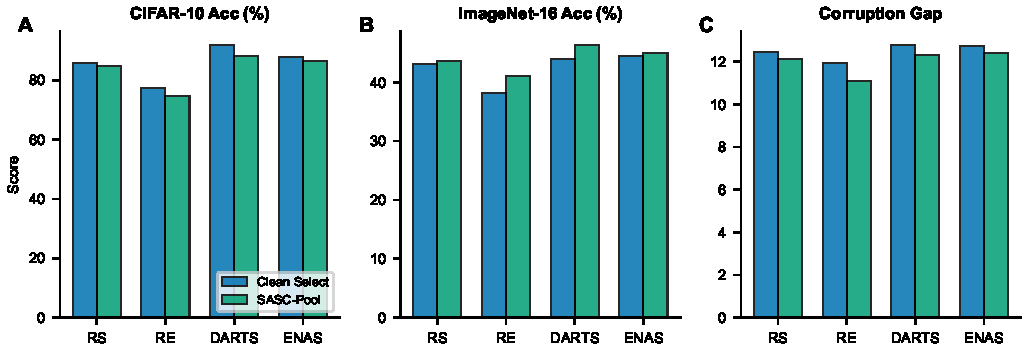
\includegraphics[width=\linewidth]{../figures/nas_algorithm_eval.pdf}
    \caption{\textbf{End-to-end NAS algorithm evaluation.} For each algorithm, clean selection (blue) vs.\ SASC-Pool (green) on the top-10 from the algorithm's candidate pool. SASC-Pool consistently improves cross-domain generalization (B) and reduces the Corruption Gap (C).}
    \label{fig:nas_eval}
\end{figure*}

\subsection{SASC-Pool Stability}
\label{sec:pool_stability}

A practical concern is whether pool-based normalization is stable when the candidate pool is small or biased.
Figure~\ref{fig:stability} shows the overlap between SASC-Pool's top-10 (from random pools of varying sizes) and SASC-Global's top-100 over the full space.
At pool sizes of $\geq$1,000, SASC-Pool reliably identifies architectures that the global oracle would also select (61\% $\pm$ 22\% overlap).
At pool size 5,000, overlap reaches 100\%.
Importantly, typical NAS algorithms explore pools of 200--1,000 architectures, placing them in the convergent regime.

\begin{figure}[t]
    \centering
    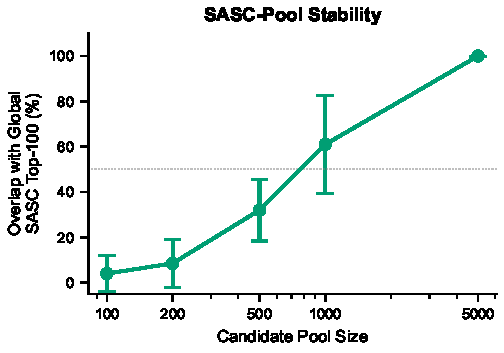
\includegraphics[width=0.85\linewidth]{../figures/sasc_stability.pdf}
    \caption{\textbf{SASC-Pool stability.} Overlap between pool-based and global SASC selections as a function of candidate pool size. SASC-Pool converges to the global optimum with pools $\geq$1,000 architectures.}
    \label{fig:stability}
\end{figure}

\subsection{Architecture Properties and Robustness}
\label{sec:arch_properties}

Figure~\ref{fig:arch_props} analyzes how architectural choices affect corruption robustness.
Skip connections show a positive correlation with \cg ($\rho = 0.27$), counter-intuitively suggesting that while skips aid clean accuracy, they do not proportionally improve robustness.
The number of ``none'' (disconnected) operations is the strongest predictor of both low clean accuracy ($\rho = -0.85$) and low \cg ($\rho = -0.95$): trivially simple architectures are uniformly fragile.
3$\times$3 convolutions contribute most to both clean accuracy and robustness, consistent with findings from RobNet~\cite{guo2020robnet}.

\begin{figure}[t]
    \centering
    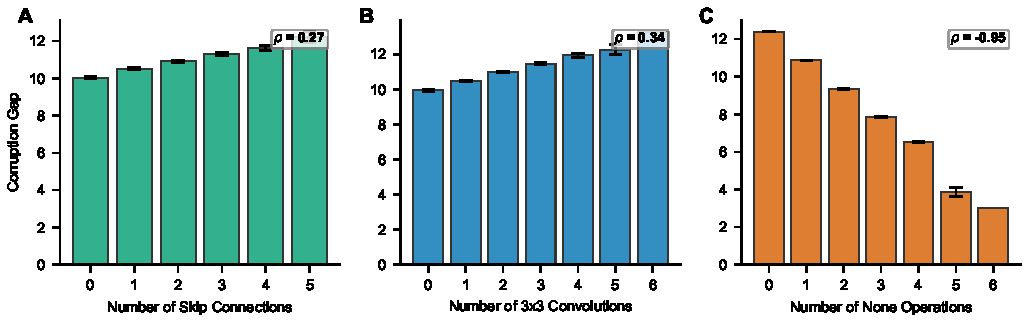
\includegraphics[width=\linewidth]{../figures/arch_properties.pdf}
    \caption{\textbf{Architecture properties vs.\ Corruption Gap.} (A) Skip connections, (B) 3$\times$3 convolutions, and (C) none operations. The number of 3$\times$3 convolutions is the strongest positive predictor of robustness.}
    \label{fig:arch_props}
\end{figure}

\subsection{Per-Corruption Analysis}

Figure~\ref{fig:radar} shows per-corruption-category performance for the three main strategies.
Clean selection achieves uniformly high corrupted accuracy (76.8--77.8\%) but with the highest \cg, indicating that its advantage is due to high clean accuracy rather than genuine robustness.
SASC-Global achieves 75.4--76.3\% across all corruption categories with more balanced performance and lower \cg.

\begin{figure}[t]
    \centering
    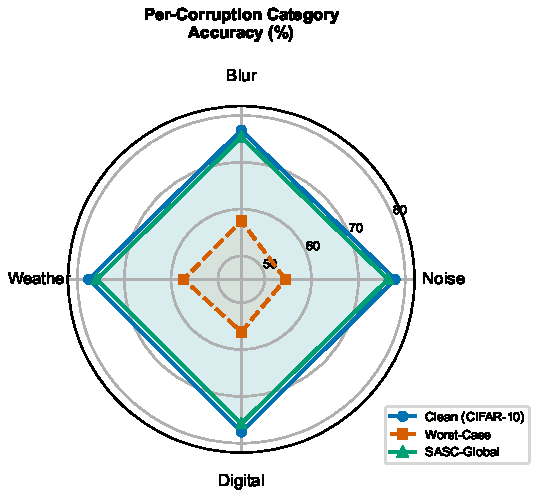
\includegraphics[width=0.85\linewidth]{../figures/corruption_radar.pdf}
    \caption{\textbf{Per-corruption category accuracy} for top-100 selected architectures. SASC-Global (green) provides balanced performance across all four corruption categories.}
    \label{fig:radar}
\end{figure}

\subsection{SASC Sensitivity Analysis}
\label{sec:sensitivity}

Figure~\ref{fig:sensitivity} shows SASC-Global performance as a function of the weighting parameters $\alpha$ (clean), $\beta$ (cross-dataset), and $\gamma$ (robustness).
Clean accuracy monotonically increases with $\alpha$, while the optimal corrupted accuracy occurs at $\alpha \approx 0.6$--$0.7$.
The default $\alpha{=}0.4, \beta{=}0.3, \gamma{=}0.3$ provides a balanced operating point; practitioners can adjust weights based on deployment requirements.

\begin{figure}[t]
    \centering
    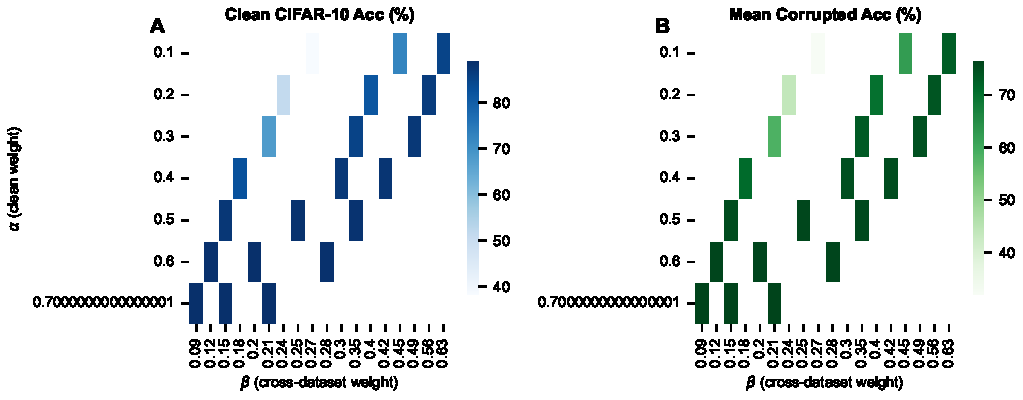
\includegraphics[width=\linewidth]{../figures/sasc_sensitivity.pdf}
    \caption{\textbf{SASC sensitivity analysis.} (A) Clean CIFAR-10 accuracy and (B) mean corrupted accuracy as functions of the clean weight $\alpha$ and cross-dataset weight $\beta$.}
    \label{fig:sensitivity}
\end{figure}

\subsection{Real CIFAR-10-C Validation}
\label{sec:real_validation}

To validate our simulated corruption analysis, we trained 46 architectures from scratch on CIFAR-10 for 50 epochs and evaluated each on all 15 CIFAR-10-C corruptions at 5 severity levels (75 conditions per architecture) using A10G GPUs.
Of the 46, 28 are functional (${>}15\%$ clean accuracy) and 18 are degenerate controls (all-none, all-skip, all-pool operations).

\paragraph{Real corruption gaps confirm the central thesis.}
Table~\ref{tab:real_results} shows that the highest-accuracy architectures exhibit Corruption Gaps of 48--51, meaning they lose roughly half their clean accuracy under corruption.
The Spearman correlation between clean accuracy and Corruption Gap among functional architectures is $\rho = 0.58$ ($p = 0.001$), confirming that architectures optimized for clean accuracy are \emph{not} proportionally robust.
Top-10 overlap between rankings by clean accuracy and by mean corrupted accuracy is only \textbf{60\%}, demonstrating real ranking instability on the corruption axis.

\begin{table}[t]
\centering
\caption{\textbf{Real CIFAR-10-C results} for representative architectures. Top-5 by clean accuracy, plus the architecture with lowest CG among those above 90\% accuracy. All numbers from real training and evaluation.}
\label{tab:real_results}
\small
\setlength{\tabcolsep}{2.5pt}
\begin{tabular}{@{}lcccccc@{}}
\toprule
Arch & Clean & \cg & Noise & Blur & Weath. & Digit. \\
\midrule
11468 & \textbf{92.3} & 51.1 & 28.4 & 37.9 & 46.0 & 49.2 \\
11418 & 91.8 & 50.6 & 25.5 & 39.9 & 47.0 & 48.6 \\
3968  & 91.1 & 51.0 & 27.2 & 36.8 & 46.1 & 47.3 \\
11593 & 91.1 & \textbf{48.8} & 27.9 & \textbf{41.6} & \textbf{48.3} & 47.7 \\
11093 & 91.0 & 50.5 & 26.4 & 37.9 & 46.7 & 47.5 \\
\midrule
11718$^\dagger$ & 90.7 & \textbf{48.2} & \textbf{33.4} & 38.5 & 47.1 & \textbf{48.6} \\
\bottomrule
\end{tabular}
\vspace{1pt}
{\raggedright\scriptsize $^\dagger$All-conv3x3 architecture (6/6 edges); lowest CG among top-15 by clean accuracy.\par}
\end{table}

\paragraph{Severity-dependent degradation.}
The top-5 architectures drop from 60.5\% mean accuracy at severity 1 to 26.4\% at severity 5---a 34-point collapse.
Noise corruptions are the most damaging (mean 27\% for top-5), followed by blur (38\%), digital (48\%), and weather (47\%).
This heterogeneity across corruption categories further motivates multi-axis evaluation.

\paragraph{Architectural insights.}
Architecture 11718 (6$\times$ \texttt{conv3x3}, 0 skip connections) achieves the lowest Corruption Gap (48.2) among the top-15 architectures despite not having the highest clean accuracy, confirming that operation diversity---not just raw capacity---affects robustness.
Figure~\ref{fig:real_validation} shows the full scatter plot and per-category breakdown.

\begin{figure}[t]
    \centering
    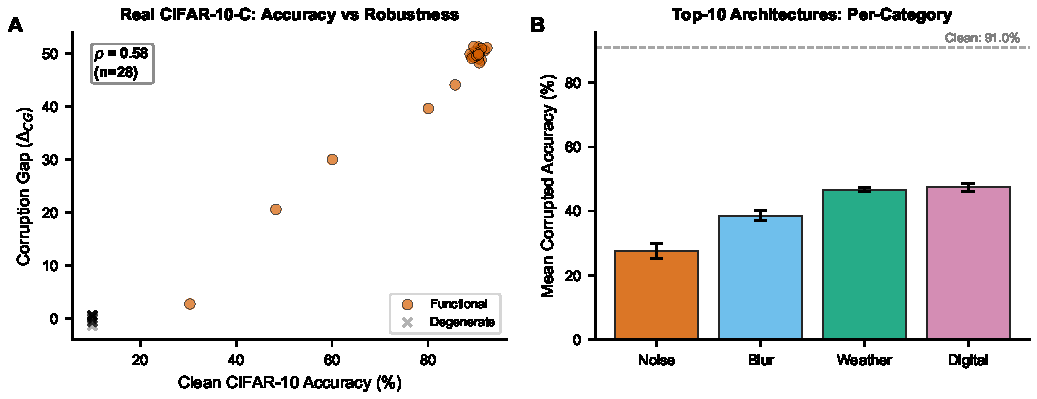
\includegraphics[width=\linewidth]{../figures/real_cifar10c_validation.pdf}
    \caption{\textbf{Real CIFAR-10-C validation.} (A) Clean accuracy vs.\ Corruption Gap for 46 real-trained architectures ($\rho = 0.58$). (B) Per-corruption category accuracy for the top-10 architectures, showing noise as the most damaging category.}
    \label{fig:real_validation}
\end{figure}
